%%%% ijcai21-multiauthor.tex

\typeout{IJCAI--21 Multiple authors example}

% These are the instructions for authors for IJCAI-21.

\documentclass{article}
\pdfpagewidth=8.5in
\pdfpageheight=11in
% The file ijcai21.sty is NOT the same than previous years'
\usepackage{ijcai21}

% Use the postscript times font!
\usepackage{times}
\renewcommand*\ttdefault{txtt}
\usepackage{soul}
\usepackage{url}
\usepackage[hidelinks]{hyperref}
\usepackage[utf8]{inputenc}
\usepackage[small]{caption}
\usepackage{graphicx}
\usepackage{amsmath}
\usepackage{booktabs}
\urlstyle{same}

%START: added by zhbli
\usepackage{subfigure}  % show sub-figure
\usepackage{algorithm}  % for algrithm
\usepackage{algorithmic}  % for algrithm
\usepackage{multirow}  % for multirow command used in the table
\usepackage{amsfonts}  % for mathbb
\usepackage{color,xcolor}  % 用于改变字体颜色
\usepackage{amssymb}  % 用于打对号
\usepackage{amsfonts}  % 用于 mathbb
%\usepackage{cite}  % 用于引用多篇文献
\newcommand{\eg}{e.g.}
\newcommand{\ie}{i.e.}
%\usepackage{float}  % 如果你确实需要把图片放在当前位置,不容改变,可以用float宏包的[H]选项。
%\usepackage[section]{placeins}  % 如果希望避免浮动体跨过 \section,可以使用 placeins 宏包。
%END: added by zhibi

% the following package is optional:
%\usepackage{latexsym}

% Following comment is from ijcai97-submit.tex:
% The preparation of these files was supported by Schlumberger Palo Alto
% Research, AT\&T Bell Laboratories, and Morgan Kaufmann Publishers.
% Shirley Jowell, of Morgan Kaufmann Publishers, and Peter F.
% Patel-Schneider, of AT\&T Bell Laboratories collaborated on their
% preparation.

% These instructions can be modified and used in other conferences as long
% as credit to the authors and supporting agencies is retained, this notice
% is not changed, and further modification or reuse is not restricted.
% Neither Shirley Jowell nor Peter F. Patel-Schneider can be listed as
% contacts for providing assistance without their prior permission.

% To use for other conferences, change references to files and the
% conference appropriate and use other authors, contacts, publishers, and
% organizations.
% Also change the deadline and address for returning papers and the length and
% page charge instructions.
% Put where the files are available in the appropriate places.

\title{Video-Agnostic Perturbations: Efficient Targeted Attacks \\ for Siamese Visual Tracking}

\author{
Zhenbang Li$^1$\and
Jin Gao$^2$\footnote{Corresponding Author}\and
YaYa Shi$^{2,3}$\and
Bing Li$^4$\and
Pengpeng Liang$^5$\And
Weiming Hu$^6$\\
\affiliations
$^1$First Affiliation\\
$^2$Second Affiliation\\
$^3$Third Affiliation\\
$^4$Fourth Affiliation\\
\emails
\{first, second\}@example.com,
third@other.example.com,
fourth@example.com
}

\begin{document}

\maketitle

\begin{abstract}

Siamese trackers are shown to be vulnerable to adversarial attacks recently. However, the existing attack methods craft the perturbations for each video independently, which comes at a non-negligible computational cost. The question is what if we can not get access to the limited computational resources in the real-world online-tracking phase.

In this paper, we show the existence of video-agnostic perturbations that can enable the targeted attack, e.g., forcing a tracker to follow the ground-truth trajectory with specified offsets, to be universal and free from inference in a network. Specifically, we attack a tracker by adding a universal imperceptible perturbation to the template image and pasting a \textit{fake target}, i.e., a small universal adversarial patch, into the search images adhering to the predefined trajectory, so that the tracker outputs the location and size of the \textit{fake target} instead of the real target. Our approach allows perturbing a novel video to come at no additional cost except the mere addition and pasting operations -- and not require gradient optimisation or network inference. Experimental results on several datasets demonstrate that our approach can effectively fool the Siamese trackers in a targeted attack manner. We will make our code publicly available.

\end{abstract}

\section{Introduction}

\begin{figure}
\centering
\subfigure{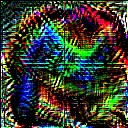
\includegraphics[width=0.2\textwidth]{images/x.jpg}} \qquad
\subfigure{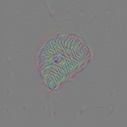
\includegraphics[width=0.2\textwidth]{images/z.jpg}}
\caption{Left: search patch. Right: template disturb.}
\end{figure}

Object tracking refers to the task of sequentially locating a specified moving object in a video, given only its initial state. Recently, Siamese networks \cite{ATOM} \cite{SiamFC} have demonstrated a significant improvement in object tracking performances. Siamese trackers formulate the visual object tracking problem as learning cross-correlation similarities between a target template and a search region. Tracking is then performed by finding the target object from the search image region by computing the highest visual similarity.

Recently, the robustness of Siamese trackers have recently attracted a lot of attention \cite{TemporallyTransferablePerturbations} \cite{efficient} \cite{SPARK}. Despite the impressive performance of Siamese architectures on challenging visual object tracking task, these trackers were shown to be highly vulnerable to perturbations.
\cite{TemporallyTransferablePerturbations} \textcolor{black}{propose a framework to generate a single temporally transferable adversarial perturbation from the object template image only. This perturbation can then be added to every search image to adversarially attack the subsequent video frames.}
\cite{efficient} \textcolor{black}{present an end-to-end network FAN (Fast Attack Network) that uses a novel drift loss combined with the embedded feature loss to attack the Siamese network based trackers.}
\cite{SPARK} \textcolor{black}{propose the spatial-aware online incremental attack (a.k.a. SPARK) that performs spatial-temporal sparse incremental perturbations online and makes the adversarial attack less perceptible.}

All the above methods can fool object trackers successfully. However, these attack methods craft the perturbations for each video independently, which comes at a non-negligible cost.
\textcolor{black}{Can we find the universal perturbations that fool a state-of-the-art deep Siamese trackers on all natural videos? We show in this paper the existence of such universal perturbations that cause the tracker to track object along any specified trajectory.}
Specifically, we aim to attack the tracker by adding an imperceptible perturbation to the template image and pasting a \textit{fake target}, i.e., a small adversarial patch into the search image adhering to the predefined trajectory, so that tracker outputs the location/size of the fake target instead of the real target.
\textcolor{black}{Different from the existing attack methods which are intrinsic dependent on videos, we generate the perturbations that can fool the network on most natural videos. Perturbing a new target then only involves the mere addition/paste operation of the universal perturbations to the template/search image -- and does not require solving an optimisation problem/gradient computation.}
Overall, our contributions can be summarized as follows:
\begin{itemize}
\item We show the existence of universal video-agnostic perturbations for state-of-the-art deep Siamese trackers. To the best of our knowledge, this is the first work to perform universal targeted attack against the visual object tracking task.
\item We propose an end-to-end pipeline to generate the universal perturbations using large scale object tracking dataset.
\item Unlike most existing attack methods which only attack the classification branch of the tracker, we simultaneously manipulate the classification and bounding box regression result of the Siamese tracker.
\item Experiment results on OTB2015 \cite{OTB}, GOT-10k \cite{GOT-10k} and LaSOT \cite{GOT-10k} datasets demonstrate that our method can effectively fool the Siamese trackers in a targeted attack manner, which comes at virtually no cost.
\end{itemize}

\section{Related Work}

\subsection{Visual Object Tracking}

Visual object tracking is a fundamental problem in computer vision, estimating the position of a template cropped from the first frame of a video in each of the subsequent video frames.
The state-of-the-art trackers can be roughly summarized to three categories, including correlation filter-based, classification \& updating-based and Siamese network-based trackers.
Recently, Siamese networks \cite{SiamRPN} \cite{SiamRPN++} have demonstrated a significant improvement in object tracking performances. Siamese trackers formulate the visual object tracking problem as learning cross-correlation similarities between a target template and a search region. Tracking is then performed by finding the target object from the search image region by computing the highest visual similarity.
In particular, SiamRPN \cite{SiamRPN} consists of Siamese subnetwork for feature extraction and region proposal subnetwork including the classification branch and regression branch. In the inference phase, the proposed framework is formulated as a local one-shot detection task.
SiamRPN++ \cite{SiamRPN++} breaks the restriction of strict translation invariance through a simple yet effective spatial aware sampling strategy and successfully train a ResNet-driven Siamese tracker with significant performance gain.
SiamFC++ \cite{SiamFC++} is designed by introducing both classification and target state estimation branch, classification score without ambiguity, tracking without prior knowledge, and estimation quality score.
In our experiments, we will focus on the SiamFC++ tracker due to its popularity in real-world applications. Nevertheless, we will study the transferability of our generated adversarial attacks to other trackers.

\subsection{Adversarial Attack}

Adversarial attacks were first investigated in \cite{intriguing} to identify the vulnerability of modern deep networks to imperceptible perturbations in the context of image classification.
Recent studies also emerge to investigate the adversarial attacks to other diverse types of tasks, e.g., natural language processing \cite{generating}, speech recognition \cite{imperceptible} and object detection \cite{wei2019transferable}.
Scenarios of possible adversarial attacks can be categorized along different dimensions.

\subsubsection{Imperceptible Perturbation v.s. Adversarial Patch}

The imperceptible perturbations most commonly modify each pixel by on a small amount and can be found using a number of optimisation strategies such as L-BFGS \cite{intriguing}, Fast Gradient Sign Method (FGSM) \cite{FGSM}, and PGD \cite{PGD}.
Different from the imperceptible perturbation, the adversarial patch is extremely salient to a neural network. The adversarial patch can be placed anywhere into the input image, and causes the network to misbehave.
To the best of our knowledge, we are the first to attack object trackers utilizing both the imperceptible perturbation and the adversarial patch together, which are jointly trained in an end-to-end manner.
Note that our adversarial patch works in the network domain instead of the image domain. In the network-domain case, the noise is allowed to take any value and is not restricted to the dynamic range of images, while in the image domain case the noise is kept to the dynamic-range of images.

\subsubsection{Non-Targeted Attack v.s. Targeted Attack}

In the case of non-targeted attack, the adversary's goal is to cause the network to predict any incorrect label and the specific incorrect label does not matter.
In the case of targeted attack, the adversary aims to change the network's prediction to some specific target label. For the video object tracking task, the targeted attack aims to intentionally drive trackers to output desired object positions specified by the targeted trajectory.

\subsubsection{Non-Universal Attack v.s. Universal Attack}

In the case of non-universal attack, the perturbations are specifically crafted of each data point independently, while the universal attack seeks a single perturbation that fools the network on most data points.
In this paper, we perform the universal attack for Siamese tracker.

\subsection{Adversarial Attack in Object Tracking}

Recently, there are several explorations of the adversarial attacks on the visual object tracking task. For example, PAT \cite{PAT} generates physical adversarial textures visa white-box attack to let the tracker lock on the texture when a tracked object moves in front of it. However, PAT validates its method by attacking a light deep regression tracker, i.e., GOTURN \cite{GOTURN} that has low tracking accuracy on modern benchmarks. In this paper, we aim to attack the state-of-the-art trackers based on the Siamese networks.
RTAA \cite{RTAA} takes temporal motion into consideration when generating lightweight perturbations over the estimated tracking results frame-by-frame. However, RTAA only performs the untargeted attack for tarckers, which causes the adversarial trajectory to deviate from the original trajectory of an object. In this paper, we focus on the more challenging targeted attack for object tracking.
SPARK \cite{SPARK} computes incremental perturbations by using information from the past frames to perform targeted attack against Siamese trackers. However, SPARK needs to generate the adversarial example for every search image in a video, which is time-consuming and ill-suited to attack an online visual tracking system in real time. In this paper, we propose universal perturbations which allow perturbing a novel video to come at no additional cost except the mere addition and pasting operations.

\begin{figure*}[t]
\centering
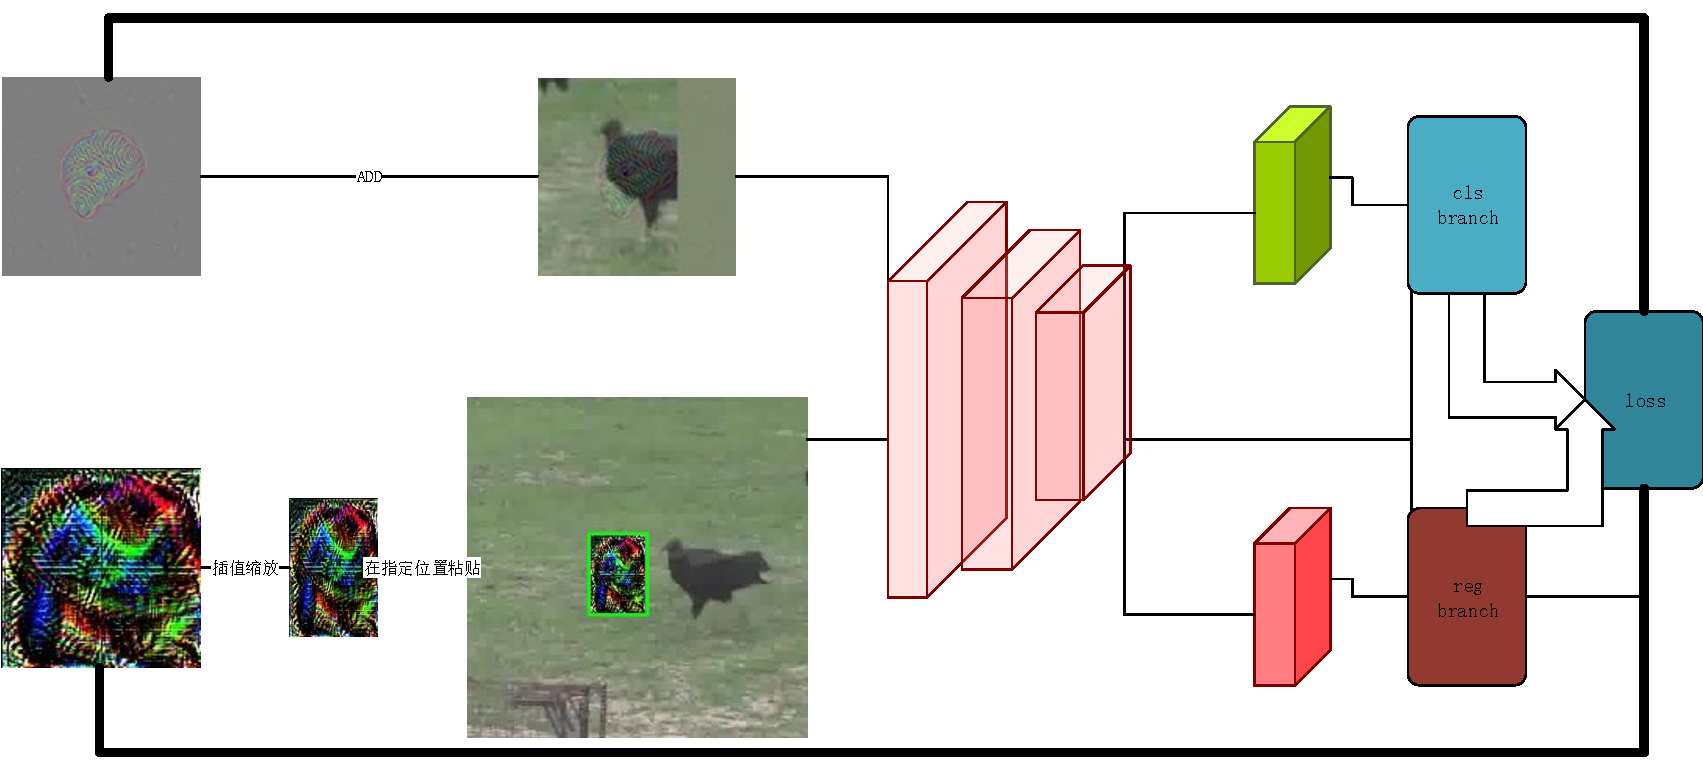
\includegraphics[width=0.8\textwidth]{images/network.pdf}
\caption{network structure}
\end{figure*}

\section{Method}

\textcolor{black}{In this section, we introduce our universal targeted attack framework for object trackers based on Siamese networks. We aim to attack the tracker by adding an imperceptible perturbation to the template image and pasting a \textit{fake target}, i.e., an adversarial patch into the search image adhering to the predefined trajectory, so that the tracker outputs the location of the fake target instead of the real target. Below, we formalize the task of performing universal targeted attacks on an object tracker, and then introduce our perturbation strategy in detail.}
 
\subsection{Problem Definition}

Let $V=\{I_i\}_1^T$ denote the frames of a video sequence of length $T$.
$B^{gt}=\{b^{gt}_i\}_1^T$ is used to represent the target's ground-truth position in each frame.
The visual object tracking will predict the position $B^{pred}=\{b^{pred}_i\}_1^T$ of this target in the subsequent frames when given its initial state.
In SiamFC++ \cite{SiamFC++}, the tracker first transforms the reference frame $I_1$ and annotation $b_1^{gt}$ to get an template image $\textbf z$, and transforms the candidate frame $I_i$ to get the search image $\textbf x_i$ centered at the position obtained in the previous frame.
At each time-step, the template image $\textbf z$ and the search image $\textbf x_i$ are first passed individually through a shared backbone network, and the resulting features are processed by some non-shared layers and fused by depth-wise separable correlation. The fused features then act as input to a head network, which predicts a classification map $\textbf{C}$, a bounding box regression map $\textbf{R}$, and a quality assessment map $\textbf{Q}$. In short, $\textbf C$ encodes the probability of each spatial position to contain a the target, $\textbf R$ regresses the bounding box position of the target, and $\textbf Q$ predicts the target state estimation quality. The final bounding box is then generated according to $\textbf{C}$, $\textbf{R}$ and $\textbf{Q}$.

Formally, we aim to train an imperceptible perturbation $\delta$ for the template image $\textbf z$, and an adversarial patch $p$ for the search image $\textbf x$. After adding $\delta$ to $\textbf z$ and pasting the fake target $p$ to $\textbf x$, the tracker outputs the location of the adversarial patch instead of the real target.
Both $\delta$ and $p$ are universal (i.e., video-agnostic), which means perturbing a new video only involves the mere addition/paste of the perturbations to the template/search image -- and does not require solving an optimisation problem/gradient computation.

\begin{table*}
\centering
\resizebox{\textwidth}{!}{%
\begin{tabular}{c|ccccccccccccccccc}
\toprule
iter num &  0    &  1    &  2    &  4    & 8   & 16  & 32  & 64  & 128 & 256  & 512   & 1024  & 2048  & 4096  & 8192  & 16384 & 32768 \\ \midrule
FGT-AO   & 0.004 & 0.002 &0.002 & 0.002 &0.002&0.002&0.003&0.007&0.042& 0.299& 0.668 & 0.746 & 0.781 & 0.798 & 0.820 & 0.821 & 0.818 \\
FGT-SR-50& 0.000 & 0.000 &0.000 & 0.000 &0.000&0.000&0.001&0.005&0.044& 0.335& 0.749 & 0.822 & 0.855 & 0.872 & 0.895 & 0.897 & 0.890 \\ \midrule
GT-AO    &  0.760& 0.757 &0.756 & 0.757 &0.757&0.758&0.759&0.753&0.720& 0.474& 0.150 & 0.095 & 0.071 & 0.041 & 0.032 & 0.032 & 0.035 \\
GT-SR-50 &  0.897& 0.894 &0.891 & 0.893 &0.891&0.893&0.896&0.888&0.852& 0.559& 0.164 & 0.098 & 0.066 & 0.031 & 0.021 & 0.022 & 0.023 \\ \midrule
SSIM     &  1.00 & 1.00  & 1.00 & 1.00  &1.00 &0.99 & 0.99& 0.97& 0.93& 0.86 & 0.86  & 0.87  & 0.88  & 0.88  & 0.88  & 0.88  & 0.88  \\
MSE      &  0.00 & 0.51  & 0.26 & 0.32  & 0.37& 0.48& 0.84& 2.03& 5.65&15.10 & 25.43 & 23.70 & 21.89 & 20.69 & 20.49 & 20.03 & 20.87 \\ \bottomrule
\end{tabular}%
}
\caption{Influence of Training Iterations}
\label{tab:iter}
\end{table*}

\subsection{Generating Universal Perturbations}

In this subsection, we show how to train the universal perturbations $(\delta, p)$ for Siamese trackers.
During the $k$-th iteration of training, a video $V=\{I_i\}_1^T$ is randomly select from the training dataset $\mathcal V$. Assuming the template perturbation at the $k$-th iteration is $\delta_k \in \mathbb{R}^{127\times 127 \times 3}$, and the adversarial patch is $p_k \in \mathbb{R}^{128\times 128\times 3}$. We first randomly pick two frames $I_t, I_s$ from $V$.
The clean template image $\textbf z\in \mathbb{R}^{127\times 127 \times 3}$ is generated according to $I_t$ and $b^{gt}_t$, and the perturbed template image is:
\begin{equation}
\tilde {\textbf z} = \textbf z + \delta_i.
\end{equation}
Similarly, the clean search image $\textbf x \in \mathbb{R}^{303\times 303 \times 3}$ is generated according to $I_s$ and $b^{gt}_s$.
As mentioned before, the patch is regarded as a fake target and pasted on the search image. We force the center position of the fake target to near the center position of the real target (i.e., the center of the search image) with an offset $(\Delta_x, \Delta_y)$. We set this offset to $(\pm 64, \pm 64)$. The width/height of the fake target is randomly selected between 32 pixels and 128 pixels.
The perturbed search image is generated as follows:
\begin{equation}
\tilde{\textbf x} = A(\textbf x, p_i, (l^x, l^y), (w, h)),
\end{equation}
where $(l_x, l_y)$ and $(w, h)$ represents the position and size of the fake target relative to the search image, respectively. $A$ is patch application operator \cite{patch} which first resizes the patch $p_k \in \mathbb{R}^{128\times 128\times 3}$ to $\hat{p}_k \in \mathbb{R}^{w\times h\times 3}$, and then applies the resized patch $\hat{p}_k$ to the search image $\textbf x$ at location $(l_x,l_y)$.

Subsequently, the SiamFC++ tracker $\phi(\cdot)$ takes $\tilde {\textbf x}$ and $\tilde{\textbf  z}$ as input and makes predictions as follows:
\begin{equation}
\textbf{C, R, Q} = \phi(\tilde {\textbf x}, \tilde{\textbf  z}),
\end{equation}

\subsubsection{Training Objective}

The loss function is calculated as follows:
\begin{equation}
\begin{array}{l}
\begin{aligned}
L&=\frac{\alpha}{N_{\mathrm{pos}}} \sum_{x, y} L_{\mathrm{cls}}\left(\textbf{C}_{x, y}, \textbf{C}_{x, y}^{*}\right) \\
&+\frac{\beta}{N_{\mathrm{pos}}} \sum_{x, y} \textbf{1}_{\left\{\textbf{C}_{x, y}^{*}>0\right\}} L_{\mathrm{quality}}\left(\textbf{Q}_{x, y}, \textbf{Q}_{x, y}^{*}\right) \\
&+\frac{\gamma}{N_{\mathrm{pos}}} \sum_{x, y} \textbf{1}_{\left\{\textbf{C}_{x, y}^{*}>0\right\}} L_{\mathrm{reg}}\left(\textbf{R}_{x, y}, \textbf{R}_{x, y}^{*}\right) \\
&+\eta \cdot ||\textbf z||_2^2 +  \sigma \cdot ||\textbf x||^2_2
\end{aligned}
\end{array}
\end{equation}
\textcolor{black} %(SiamFC++)
{where $\textbf{C}_{x, y}, \textbf{R}_{x, y}, \textbf{Q}_{x, y}$ represent the values of $\textbf{C}, \textbf{R}, \textbf{Q}$ at location $(x, y)$, respectively. $\textbf{C}^*, \textbf{R}^*, \textbf{Q}^*$ are the fake labels generated according to the position/size of the fake target.$\textbf 1$ is the indicator function that takes 1 if the condition in subscribe holds and takes 0 if not, $L_{\mathrm{cls}}$ denote the focal loss \cite{focal} for classification result, $L_{\mathrm{quality}}$ denote the binary cross entropy (BCE) loss for quality assessment and $L_{\mathrm{reg}}$ denote the IoU loss \cite{iou-loss} for bounding box result. Following SiamFC++, we assign 1 to $\textbf{C}_{x, y}^{*}$ if $(x, y)$ is considered as a positive sample, and 0 if as a negative sample.}

\begin{algorithm}[tb]
\caption{Example algorithm}
\label{alg:algorithm}
\textbf{Input}: Videos $V$, Siamese tracker $T$, max iteration $N$\\
\textbf{Parameter}: Universal perturbation $\delta$ and universal patch $\sigma$.\\
\textbf{Output}: Universal perturbation $\delta$ and universal patch $\sigma$.
\begin{algorithmic}[1] %[1] enables line numbers
\STATE Let $\delta=0, \sigma=0, i = 0$.
\WHILE{$i < N$}
\STATE random pick a video $v\in V$.
\STATE random pick two frames $I_i, I_j$ from $v$.
\STATE generate template image $z = f(I_i)$.
\STATE generate search image $x = f(I_j)$.
\STATE generate perturbed template image $\tilde z = z + \delta$
\STATE generate perturbed search image $\tilde x = A(x, \sigma)$
\STATE generate prediction $y = F(\tilde x, \tilde z)$
\STATE generate fake ground truth $\hat y = B(A)$
\STATE $\delta = \delta - \epsilon_1\cdot\text{sign}(\nabla_{\delta}L(y, \hat y))$
\STATE $\sigma = \sigma - \epsilon_2 \cdot \text{sign}(\nabla_{\sigma}L(y, \hat y))$
\STATE $i = i + 1$
\IF {conditional}
\STATE Perform task A.
\ELSE
\STATE Perform task B.
\ENDIF
\ENDWHILE
\STATE \textbf{return} solution
\end{algorithmic}
\end{algorithm}

\subsubsection{optimisation}

\begin{figure*}[t]
\centering
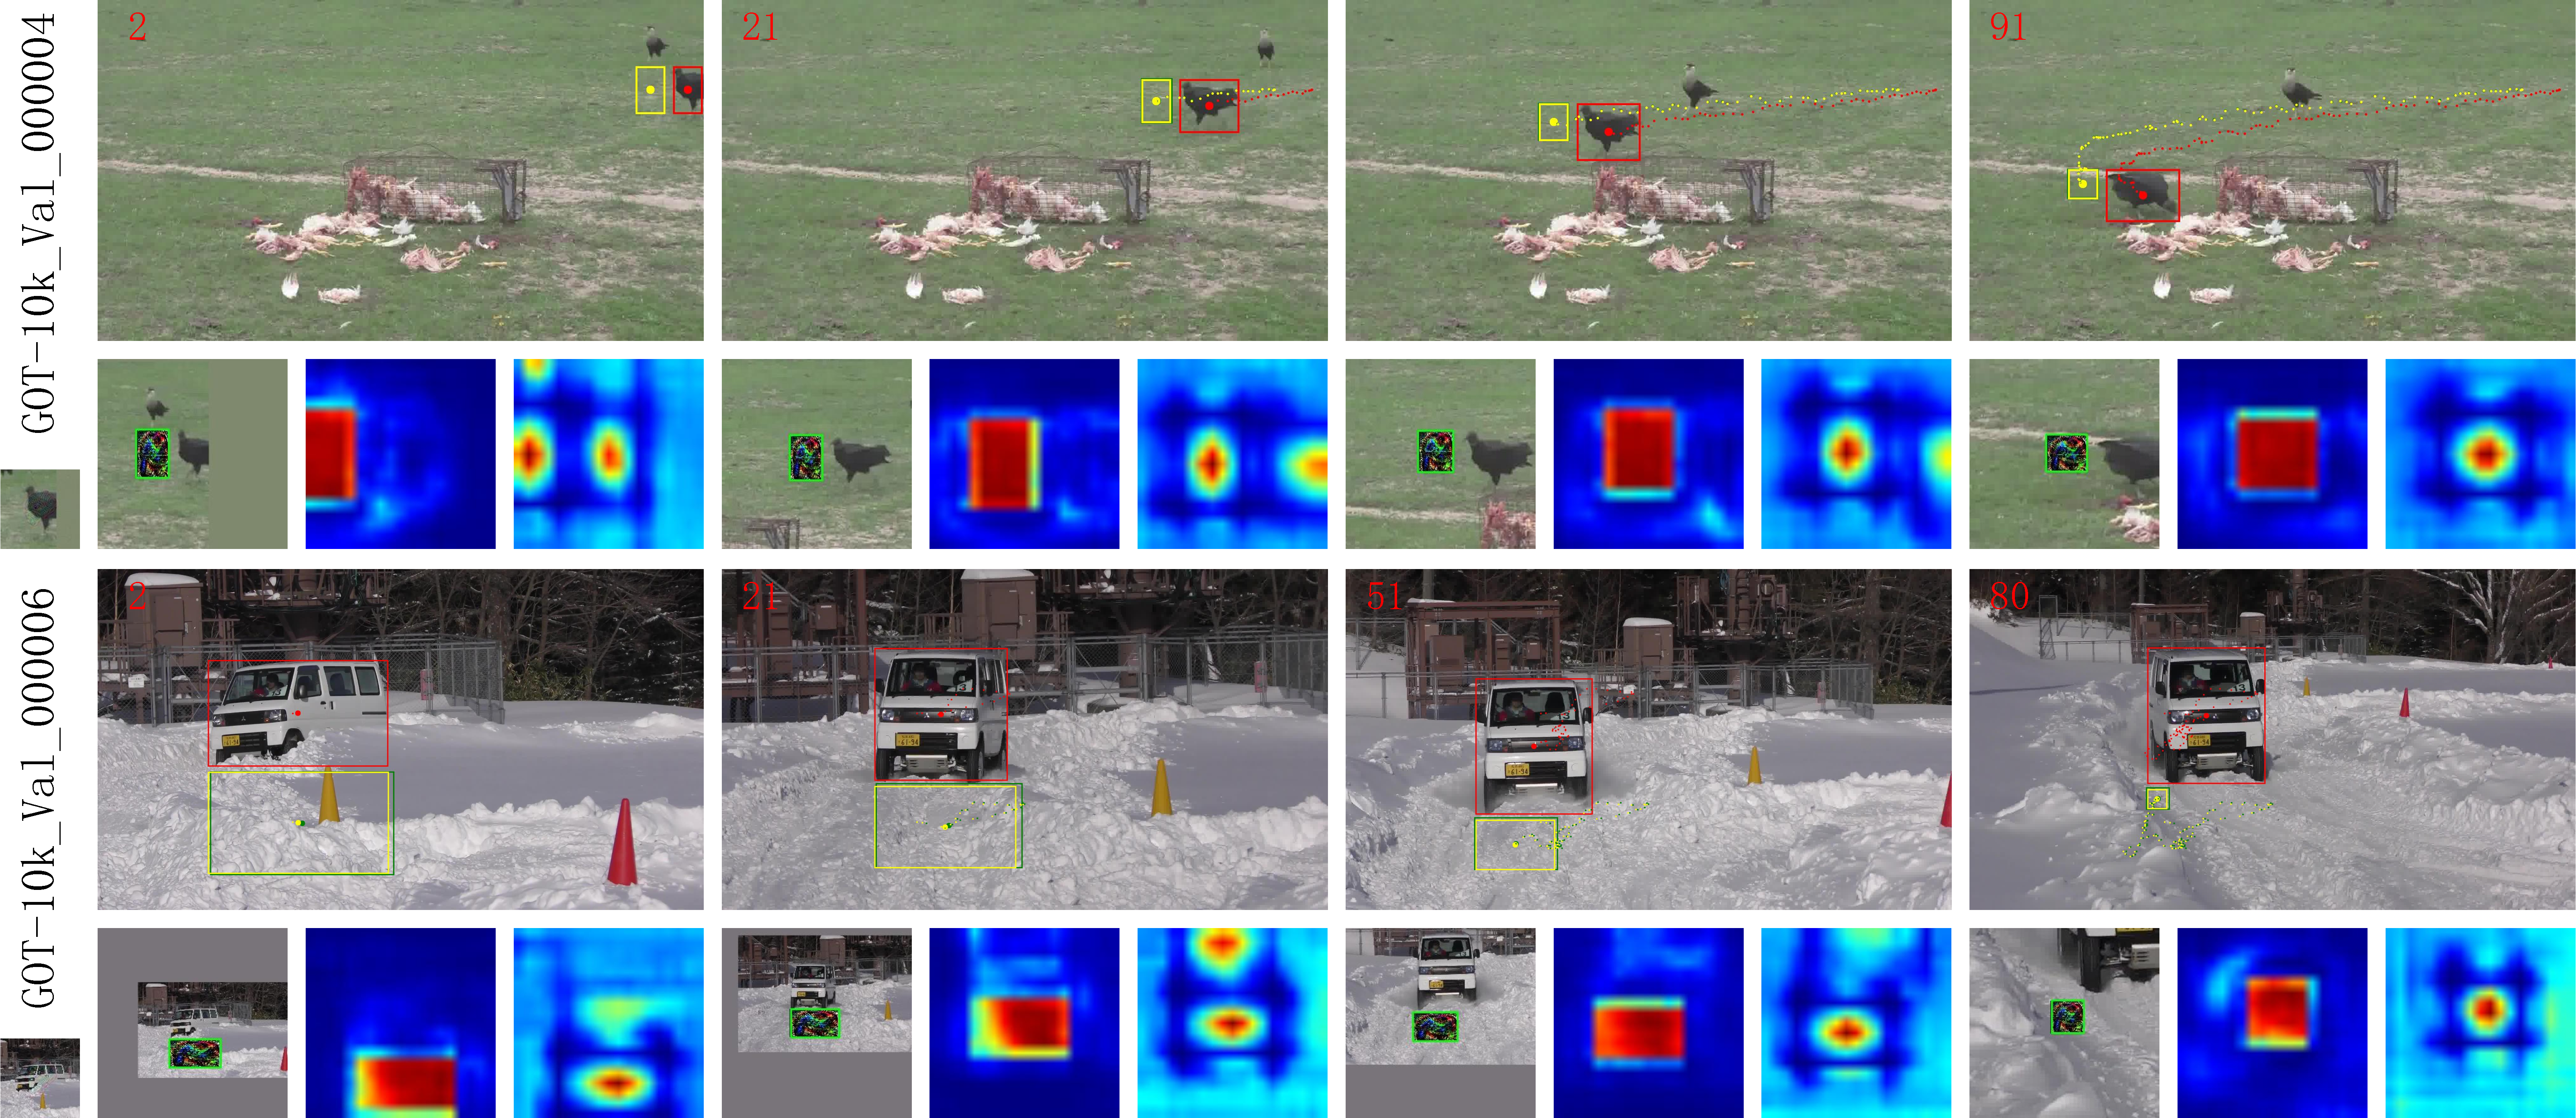
\includegraphics[width=1\textwidth]{images/vis_2.pdf}
\label{fig:vis}
\end{figure*}

At each training step, the perturbations are updated as follows:
\begin{gather}
\delta_{k+1} = \delta_{k} - \epsilon_1 \cdot \text{sign}(\nabla_{\delta_k}L)\\
p_{k+1} = p_{k} - \epsilon_2 \cdot \text{sign}(\nabla_{p_k}L)
\end{gather}
where $\epsilon_1$ is used to ensure that the perturbation added to the template image is imperceptible, and $\epsilon_2$ is used to maintain the training stability.
During training, we only optimize the values of perturbations $(\delta, p)$, and the parameters of the Siamese network remain intact.

\begin{table}[hbtp]
\centering
\resizebox{0.48\textwidth}{!}{%
\begin{tabular}{c c|c c c}
\toprule
\multicolumn{2}{c|}{Trackers} & 
\begin{tabular}{c} \textbf{SiamFC++\_} \\ \textbf{GoogLeNet} \end{tabular} &
\begin{tabular}{c} \textbf{SiamFC++\_} \\ \textbf{GT} \end{tabular} &
\begin{tabular}{c} \textbf{Ours} \\ \textbf{FGT} \end{tabular} \\
\midrule
\multirow{2}{*}{OTB-15} 
& Success   & 64.2 & 3.5 & 84.2\\
& Precision & 86.1 & 4.8 & 92.8\\
\midrule
\multirow{3}{*}{GOT-Val} 
& SR\textsubscript{.50} & 0.897 & 0.023 & 0.890\\
& AO 				   & 0.760 & 0.035 & 0.818 \\
\midrule
\multirow{4}{*}{LaSOT} 
& Prec.       & 0.514 & 0.013 & 0.820\\
& Norm. Prec. & 0.551 & 0.015 & 0.788\\
& Succ. score & 0.525 & 0.022 & 0.767\\
& Succ. rate  & 0.626 & 0.016 & 0.834\\
\midrule
\multicolumn{2}{c|}{FPS} & 58 & 58 & 58\\
\bottomrule
\end{tabular}}
\caption{Ablation study results on several benchmarks.}
\label{tab:benchmark results}
\end{table}

\subsection{Attacking the Tracker at Inference Time}

Once the the perturbations $(\delta, p)$ is trained, we can use them to perturb the template image and search images of any natural video. Both $\delta$ and $p$ are universal (i.e., video-agnostic), which means perturbing a new video only involves the mere addition/paste of the perturbations to the template/search image -- and does not require solving an optimisation problem/gradient computation.
Assume $B^{fake}=\{b^{fake}_i\}_1^{T}$ is the trajectory we hope the tracker to output.
During tracking the $i$-th frame of the video $V=\{I_i\}_1^T$, we need to transform the bounding box $b^{fake}_i$ (relative to the original frame $I_i$) into the box $\hat b_i=\{l^x_i, l^y_i, w_i, h_i\}$ relative to the search image $\textbf x_i$, and paste $p$ into $\textbf x_i$ according to $\hat b_i$:
\begin{equation}
\tilde{\textbf x}_i = A(\textbf x_i, p, (l^x_i, l^y_i), (w_i, h_i)).
\end{equation}
The tracker then takes $\tilde{\textbf z}=\textbf z+\delta$ and $\tilde{ \textbf x}_i$ as input, and the subsequent tracking procedure remains the same as SiamFC++.

\section{Experiments}

\subsection{Datasets and Implementation Details}

We use SiamFC++ as our base tracker, and the backbone Siamese network adopts GoogLeNet.
We implement our our approach in Pytorch and train our perturbations using 3 GTX 1080Ti GPUs.
We adopt GOT-10k \cite{GOT-10k}, COCO \cite{COCO}, ILSVRC-VID \cite{VID} and LaSOT \cite{LaSOT} and our training set.
We train the perturbations for 32768 iterations with a minibatch of 96 images (32 images per GPU).
The learning rate of the template perturbation $\epsilon_1$ is set to 0.1, and the learning rate of the adversarial patch is $\epsilon_2 = 0.5$.
We generate training samples following the strategy in SiamFC++.
During the training and the testing phase, the size of the template image is set to $127\times 127\times 3$, and the size of the search image is set to $303\times 303\times 3$.
In equ. ?, we set $\alpha=1, \beta=1, \gamma=1, \eta=0.005, \sigma=1e-5$.
\textbf{Datasets} We evaluate our universal perturbations on several tracking datasets: OTB2015 \cite{OTB}, GOT-10k Val \cite{GOT-10k}, and LaSOT \cite{LaSOT}.

%Although we do not need to control the weight of $x$, but in experiment we find that it will influence the stability of the training phase.
%Note that the negative pairs are not involved as part of training samples, because we always paste the fake target into the search image.
%The size of the template is 127 * 127. The size of the search image is 303 * 303 during both training and inference phase.
%we initialize our template perturbation as 0, and patch as 128. To avoid the bad influence of the rescale, which can cause the information loss, we always use the big patch. When paste onto the search image, we rescale the patch (mostly down-sample) and then paste.

\subsection{Result on Several Benchmarks}

We test our tracker on several benchmarks and results are gathered in Table \ref{tab:benchmark results}.
Note that, in the original siamfc++ paper, they test different dataset using different trained model. But we test them using one single model. So on some datasets will drop slightly.

\subsubsection{Evaluation on OTB2015 Benchmark}

As one of the most classical benchmarks for the object tracking task, the OTB benchmark provides a fair test for trackers. We conduct experiments on OTB2015 \cite{OTB} which contains 100 videos for tracker performance evaluation.
We use success rate to evaluate the performance of trackers on the OTB2015 dataset. Success rate relies on the intersection over union (IOU) of the predicted bounding box and the ground truth bounding box.
The success score relative to $B^{gt}$ on the clean videos is 0.642. The success score relative to $B^{gt}$ on the adversarial videos is 0.035. The success score relative to $B^{fake}$ on the adversarial videos is 0.842.

\subsubsection{Evaluation on GOT-10k Benchmark}

GOT-10k \cite{GOT-10k} is a recent large-scale high-diversity dataset. There is no overlap in object classes between the train/val/test splits, promoting the importance of generalization to unseen object classes.
%Because we need to use the real ground truth to generate the fake ground truth, and the fake ground truth is not available on test set, so we use the val set.
%The evaluation metric is AO and Success rate, which means ...
On GOT-10k Val set, the AO relative to $B^{gt}$ on the clean videos is 0.760. The AO relative to $B^{gt}$ on the adversarial videos is 0.023. The AO relative to $B^{fake}$ on the adversarial videos is 0.818.

\subsubsection{Evaluation on LaSOT Benchmark}

With a large number of video sequences, LaSOT (Largescale Single Object Tracking) benchmark makes it impossible for trackers to overfit the benchmark, which achieves the purpose of testing the real performance of object tracking.
Following onepass evaluation, different trackers are compared based on three criteria including precision, normalized precision and success.
The precision score relative to $B^{gt}$ on the clean videos is 0.514. The precision score relative to $B^{gt}$ on the adversarial videos is 0.013. The precision score relative to $B^{fake}$ on the adversarial videos is 0.820.

\subsection{Ablation Studies}

\subsubsection{Influence of Training Loss}

We implement a series of experiments to analyse and evaluate the contribution of each loss component.
In Table. ?, we report our results on GOT-10k val set with different combination of loss terms, where $L_{cls}, L_{quality}, L_{reg}$ represent the classification loss, the quality assessment loss and the regression loss in Equ. ?, respectively.
To summarize, while all loss terms are beneficial, the classification term is more efficient than the quality assessment term. 
%We find use three loss to train together can achieve better performance. In line one, we only train the classification branch. After adding all three losses, our attack achieve better performance. We can see that the classification loss contributes most. And the center loss contributes less.

\begin{table}[h]
\centering
\resizebox{0.4\textwidth}{!}{%
\begin{tabular}{ccc|cccc}
\toprule
$L_{cls}$ & $L_{quality}$ & $L_{reg}$ & FGT AO & FGT SR50 & GT AO & GT SR50 \\ \midrule
\checkmark   &    &    & 0.718  & 0.824    & 0.086 & 0.083   \\
   & \checkmark   &    & 0.044  & 0.044    & 0.703 & 0.842   \\
   &    & \checkmark   & 0.664  & 0.726    & 0.165 & 0.184   \\
\checkmark   & \checkmark   & \checkmark   & 0.781  & 0.855    & 0.071 & 0.066   \\ \bottomrule
\end{tabular}}
\caption{Different loss weight.}
\end{table}

\subsubsection{Influence of Training Iterations}

As shown in table \ref{tab:iter}, after approximately 30000 training iterations, the generated perturbations could fool most targets in GOT-10k Val. The AO relative to $B^{gt}$ falls down from 0.760 to 0.035. We notices that at the start of training period (when training iteration is less than 2048), the falling speed of AO relative to $B^{gt}$ is largest. This demonstrates the efficiency of our end-to-end training pipeline used to generate the adversarial perturbations.

\subsection{Transferability}

\subsubsection{Transferability of different backbone}

We evaluate the transferability of our attacks on different backbones of SiamFC++: ShuffleNet \cite{ShuffleNet} and AlexNet \cite{AlexNet}.
The experimental results are shown in Table. ?. On SiamFC++-AlexNet, the AO relative to $B^{gt}$ drops from 0.72 to 0.196, which suggests that our perturbation can still work. However, our perturbations does not generalize well on SiamFC++-ShuffleNet, which we conjecture to be due to the significant difference of the network structure between googLeNet and ShuffleNet.

% Please add the following required packages to your document preamble:
% \usepackage{graphicx}
\begin{table}[h]
\centering
\resizebox{0.4\textwidth}{!}{%
\begin{tabular}{c|ccc}
\toprule
backbone & googlenet & alexnet & ShuffleNetV2x1.0 \\ \midrule
FGT-AO   & 0.818     & 0.572   & 0.135\\
FGT-SR-50& 0.890     & 0.640   & 0.134\\ \midrule
GT-AO    & 0.035     & 0.196   & 0.554\\
GT-SR-50 & 0.023     & 0.227   & 0.656\\ \midrule
ROI-AO   & 0.760     & 0.720   & 0.766\\  
ROI-SR-50& 0.897     & 0.850   & 0.888\\ \bottomrule
\end{tabular}%
}
\caption{Different backbone}
\end{table}

\subsubsection{Transferability of different architecture}

We use AlexNet-based SiamRPN \cite{SiamRPN} and ResNet-based SiamRPN++ \cite{SiamRPN++} as black-box attack models to verify the transferability of our perturbations on different tracking architectures.
SiamRPN uses an RPN network to perform location regression and classification on the response map. SiamRPN++ performs layer-wise and depth-wise aggregation to improve accuracy. Both SiamRPN and SiamRPN++ are anchor-based methods while SiamFC++ is an anchor-free method.
The experimental results are shown in Table. ?. On SiamRPN, the success score relative to $B^{gt}$ drops from 0.666 to 0.379. On SiamRPN++, the success score relative to $B^{gt}$ drops from 0.676 to 0.518. The results show that our method can still show good transferability for different tracking architectures.

%\textbf{Definition:} Transferability can judge the perturbation generated from one can still work at another network, although the network structure is very different. As we can see, we can successfully transfer from anchor free method SiamFC++ to anchor-based tracker SiamRPN \cite{SiamRPN} with backbone alexnet and SiamRPN++ \cite{SiamRPN++} with backbone resnet 50, shows the power of our attack.

\begin{table}[h]
\centering
\resizebox{0.45\textwidth}{!}{%
\begin{tabular}{c|cc|cc}
\toprule
Trackers     & Succ-ORI & Prec-ORI & Succ-ATTACK & Precision-ATTACK \\ \midrule
siamRPN++    & 0.676   & 0.879     & 0.518       & 0.691 \\
SiamRPN      & 0.666   & 0.876     & 0.379       & 0.506 \\ \bottomrule
\end{tabular}%
}
\caption{Transferability of different architecture on OTB2015}
\end{table}

\section{Conclusion}

In this paper, we propose a universal targeted attack method for Siamese trackers. 
We aim to attack the tracker by adding an imperceptible perturbation to the template image and pasting a \textit{fake target}, i.e., a small adversarial patch into the search image adhering to the predefined trajectory, so that tracker outputs the location/size of the fake target instead of the real target. An end-to-end pipeline are proposed to train the perturbations efficiently.
Experiments on several popular datasets shows that our method can effectively fool the Siamese trackers in a targeted attack manner.

\clearpage
\bibliographystyle{named}
\bibliography{ijcai21}

\section{Useless Sentences}

\subsection{How we set identify the fake path ?}

There are several methods to control the box direction. One is to generate several pre-trained perturbations, one represents a specific direction. During testing, a best direction is selected according to the fake GT position. However, there are some disadvantages of this method:
\begin{itemize}
\item They need several pre-trained perturbations. If they want more accurate, they need more pre-train.
\item They generate the approximate trajectory.
\item They have to generate  new perturbations of A new video.
\end{itemize}
To overcome these disadvantages, we use a small patch to control the prediction. So we can make the network to predict any shape/position as what we want. And we are universal.

our loss function is:
\begin{equation}
L = \alpha \cdot L_{cls} + \beta \cdot L_{ctr} +  \gamma \cdot L_{reg} + \eta \cdot ||z||_2^2 +  \sigma \cdot ||x||^2_2
\end{equation}

We will generate the fake ground truth $GT^{\text{fake}}=\{B^{fake}_i\}_1^T$.
We will predict: $\{B^{pred}_i\}_1^T$.
The tracker is $\phi$, we get the prediction $B_i^{pred}=\phi(z, x_i)$.

$z = \tau (I_1, b^{gt}_1)\in \mathcal{R}^{127\times 127\times 3}$

$x = \tau(I_i, b_{i-1}^{pred})\in \mathcal{R}^{303\times 303 \times 3}$

at each spatial location, the classification map encodes the probability of each position to contain the target, the regression map produces a corresponding offset, and the quality assessment map give the quality. 

which predicts a classification map $\textbf{C}\in \mathbb{R}^{H\times W\times 1}$, a bounding box regression map $\textbf{R}\in \mathbb{R}^{H\times W\times 4}$, and a quality assessment map $\textbf{Q}\in \mathbb{R}^{H\times W\times 1}$.

We want them universal so that no extra time is needed.
For targeted attack, suppose a fake trajectory $GT^{\text{fake}}=\{B^{fake}_i\}_1^T$ is what we hope the tracker to output, we want to drive trackers to output desired object positions specified by the targeted trajectory. This is achieved by the patch position: We paste the patch to the specified position, and we hope the tracker prediction to the patch position (i.e., the FGT).

Then we generate the perturbed template image and search image, then we generate the fake label, then we make prediction, calculate loss, and update perturbations for one iteration.

$z = \tau (I_j, b^{gt}_j)\in \mathcal{R}^{127\times 127\times 3}$

Note that we control the $\delta$ to be small. The shape of $\delta$ is $127 \times 127 \times 3$, and the shape of the $z$ is also $127 \times 127 \times 3$.

First we generate the clean search image is cropped at the center of the target:$x = \tau(I_k, b_{k}^{gt})\in \mathcal{R}^{303\times 303 \times 3}$

Then we set up the fake box in the search image. The center position of our patch is randomly put [-64, 64] near to the real target. The size of our patch is randomly from [-32, 128], to model the different size/position of the target. So we get the fake box $\hat b$. Note that $\hat b$ is relevant to the search image.

\subsubsection{Generating the Fake Label}

According to SiamFC++, there are three labels: classification label, regression label and quality assessment label.
We generate fake ground truth $\hat y$ according to patch shape/position on the search image  used for calculate loss.
We use the position of this fake GT to generate the $\hat y$.
We need the network prediction close to the FGT.
Calculate the FGT box position on the search image, according to the scale.
We generate the fake label of the tracker according to the position of the fake target:
\begin{equation}
\mathcal{C^*, Q^*, T^*} = A(m),
\end{equation}
where classification GT $S_{cls} \in R^{19 \times 19 \times 1}$, where $S_{cls}(x,y)$ denotes the classification confidence score for the box at spatial position $(x,y)$. The center GT $S_{ctr} \in \mathbb{R}^{19 \times 19 \times 1}$, where $S_{ctr}(x,y)$ denotes the quality assessment score for box at $(x,y)$, and regression GT $S_{reg} \in \mathbb{R}^{19 \times 19 \times 4}$, where $S_{reg}(x,y) \in \mathbb R^{4}$ is the delta of $B^{fake}$.

and the fake label $\tilde y$

where $y$ includes three parts: classification map $CLS \in R^{19 \times 19 \times 1}$, regression map $REG \in \mathbb{R}^{19 \times 19 \times 1}$, and center map $CTR \in \mathbb{R}^{19 \times 19 \times 4}$.

\subsubsection{Loss Function}

We use the trained network of SiamFC++ \cite{SiamFC++}.
It is an anchor free method for tracking. It contains three losses to train the tracker: classification loss, center loss and regression loss.

\subsection{Abstract}

In this paper, we propose a new method to attack the Siamese trackers. 
We \textbf{first} propose the \textbf{universal} attack for Siamese trackers, we achieve it by use the small distribution on the template image and use the patch on the search image.
We use a \textbf{fake target}, i.e., a small patch onto the search image, to guide the tracker to prediction badly.
We not only to attack by the fake target, we also manipulate the template image to boost the performance.
Different from the existing tracker attack method, we can not only control the trajectory of the target, but also the size of the target.
Our code is public at https://github.com/lizhenbang56/Universal-Targeted-Attacks-for-Siamese-Visual-Tracking
\textit{(D PATCH) Unlike the original adversarial patch that only manipulates image-level classifier, our patch simultaneously attacks the bounding box regression and object classification so as to disable their predictions.}
We propose a systematic algorithm for computing universal perturbations, and show that state-of-the-art Siamese trackers are highly vulnerable to such perturbations.

In SiamFC++, the tracker $\phi(\cdot)$ first transforms the reference frame $I_1$ and annotation $b_1$ to get an template image $z = \tau (I_1, b^{gt}_1)\in \mathcal{R}^{127\times 127\times 3}$, and searches a large area in the candidate frame $I_i$ to get the search image $x = \tau(I_i, b_{i-1}^{pred})\in \mathcal{R}^{303\times 303 \times 3}$ centered at the position obtained in the previous frame.
Then, we add the template perturbation onto the template image:
\begin{equation}
\tilde z = z + \delta
\end{equation}
Then, we calculate the box $\hat b$ onto the search image according to FGT onto the original iamge $b^{fake}_i$, then we resize the patch using that box, then put the fake patch onto the search image according to FGT:
\begin{equation}
\tilde x = A(x, p_i, \hat b)
\end{equation}
Then, we run the tracker and get the prediction. According to SiamFC++, the result of classification map and the center map is multiplied, then add the cosine window to find the best position. Then the best box according to this position is selected as the final box.

\textbf{What is attack?}

Specifically, by adding such a quasi-imperceptible perturbation to template image and a small patch on the search image, the bounding box estimated by the Siamese trackers is changed from the real target to the fake patch. Such perturbations are dubbed universal, as they are image-agnostic.

\textcolor{red}{(Adversarial patch) In this work we explore what is possible if an attack no longer restricts themselves to imperceptible changes. Instead, this attack generates an image-independent patch for the search image, and an image-independent small perturbations for the target image. The patch can then be placed anywhere within the filed view of the tracker, and causes the tracker to output a targeted position.}

Specifically, we use two forms of perturbations together to achieve this goal: Unseen small perturbations on the search image and small patch on the search image. We regard the patch as a fake target, and we want our tracker to track this fake patch target. We train our perturbations as write-box attack using FSGM \cite{FGSM} method.

The patch is powerful, it is used to point out the position and size need to track.

What we do is the targeted attack, which means the tracker follows a new trajectory. Specifically, we patch a fake target.

We perform a good solution, use unseen small perturbations on the search image and small patch on the search image to attack. / We propose an algorithm for finding such perturbations. The algorithm seeks a universal perturbation for a ...

\subsection{Generating Fake Trajectories}

We need to set specific trajectory for the video frames in the dataset to achieve targeted attack.
For targeted attacks, we need to generate a fake trajectory: The definition of the fake ground truth: ... We can set the fake ground truth as what we want.
The goal of the fake ground truth: we hope the tracker predict results similar to the fake ground truth.
During set the fake ground truth, we must guarantee the following:

\begin{itemize}
\item The fake ground truth at the first frame is close enough to the real ground truth, otherwise, we do not know where is the fake target.
\item To model the size change of the \textbf{fake target} $\tilde T$, we let the fake target size change from the original real target $T$ to 64*64 in the original image.
\item The fake target needs to near to the real target all the time, because there are chances to jump between each other.
\item Never overlap between to box $B^f_i$ and $B^r_i$ to make sure the patch can not cover the real target appearance.
\end{itemize}

\textbf{Our solution to set the fake path} We let the fake target to run as same as the real target. To show that we can control the size of the fake target, we gradually set the patch size to 64 * 64.
\textbf{Inference} 
Initial position/size of the fake target: During tracking, the fake target ground truth box is always near the \textbf{real target} of 16 pixels (on the origin image).
The initial size of the fake target is the same as the initial size of the real target.
End size of the fake target: 64 * 64.
\textbf {position of the FGT on the search image during testing}

\subsection{Evaluation Metrics}

We get the prediction boxes $B^{\text{pred}}$. So we can evaluation the overlap between the real ground truth boxes $B^{\text{GT}}$ and the fake ground truth boxes $B^{\text{FGT}}$. If we attack successful, the AO to real ground truth will drop significantly, while the AO to fake ground truth will be high. For a bad attack, the AO to real ground truth will not drop. 

Then, we use SSIM and L2 norm to judge the perturbation on the target image is small or not. 
defination of SSIM: ... we near 0.88

\textit{Image Quality Assessment: We use Mean-SSIM to evaluate the quality of adversarial videos. Mean-SSIM calculates the average SSIM of frames in videos. The generated adversarial perturbations are difficult to be found when MeanSSIM is close to 1.(Efficient Adversarial Attacks for Visual Object Tracking)}

\subsection{Qualitative Evaluation}

\textit{Fig. \ref{fig:vis} shows examples of adversarial attacks against different videos. We can see that the template perturbation is so subtle that it is difficult to be observed by the human eye. (One-shot Adversarial Attacks on Visual Tracking with Dual Attention)} The \textbf{classification map} can show the patch position very good. The \textbf{center map} may show both the real target and the patch position. They multiplied finally.

\begin{figure}[ht]
\centering
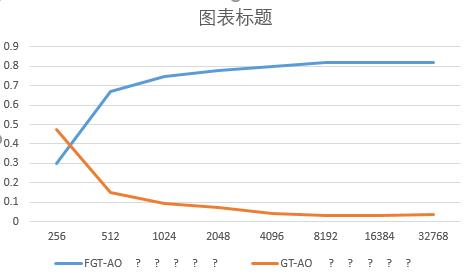
\includegraphics[width=0.4\textwidth]{images/iter.jpg}
\caption{Inflence of Training Iterations}
\end{figure}

\subsection{Related Work}

\subsubsection{Digital Attack v.s. Physical Attack}

In the case of digital attack, the adversary has direct access to the actual data fed into the model. In the case of an attack in the physical world, the adversary does not have direct access to the digital representation of provided to the model. We perform the digital attack in this paper.

In \cite{karmon2018lavan}, we can know, attack can be categorised as image domain attack and network domain attack. For image attack, the new image must at [0,255]. But for the network attack, the value can be any. We do the network domain attack, because we are more interested in investigating the blind-spots of the popular Siamese trackers.

\subsubsection{White Box Attack v.s. Black Box Attack}

In the white box scenario, the adversary has full knowledge of the model including model type, model architecture and values of all parameters and trainable weights.
Traditional adversarial attack methods include FGSM \cite{FGSM} and so on. FGSM means In the black box scenario, the adversary only have limited or no information about the model.

\end{document}
